\chapter{Background - Different Types of Networks and Their Similarities }
\label{chap:background}
In this thesis, we claim that many different types of networks are quite similar in terms of power consumption. In this chapter, we take an essentials-only look at two different types of networks with a view to establishing the similarity between them. This similarity motivates the formulation of a generalized electricity cost optimization framework. 

\section{Geo-Diverse Data Centers} Organizations like Microsoft, Facebook, Amazon and Google run a plethora of applications. Some of these applications are accessible by the general public. Google Docs is one such application. Such organizations also run private applications for the consumption of authorized internal users only. These applications run on servers that are hosted at sites called data centers.

A data center is a site that has equipment such as servers, storage and networking equipment, in addition to some allied equipment such as airconditioning and power supplies. A given data center may host only public applications, only private applications or even both. Furthermore, some public data center operators allow a client to host their own applications, whereas some only offer a fixed set of internally developed applications. For instance, one may run a custom application on a server leased on Amazon's data centers, but on the other hand, Google's search cluster only hosts the Google search application. 

Operators typically deploy multiple data centers at different geographic locations. This is done for two reasons. First, having data centers at different locations provides fault tolerance. If one site goes down for some reason, the other site may take over as a backup. Also, multiple remote sites are less likely to affected simultaneously by a natural disaster. A second reason to have multiple data centers is to have low latency to clients at different locations. For instance, Amazon has multiple data centers in different continents, thereby ascertaining that no matter where a client may be, there is an Amazon data center relatively close by compared to the case if Amazon only had one data center in the US. Figure~\ref{fig:googledcmap} shows the locations of Google's data centers across the globe (according to royal.pingdom.com as of April 2008).

\begin{figure}
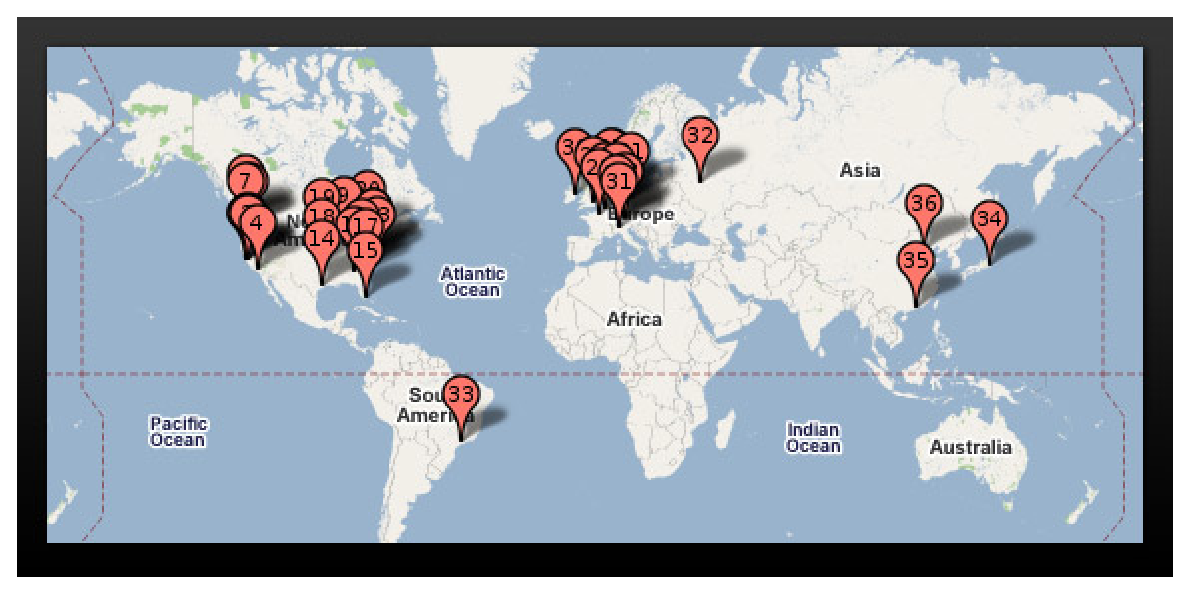
\includegraphics[width=1\textwidth]{pics/googledcmap.eps}
\label{fig:googledcmap}
\caption{Google Data Center Locations - Source: royal.pingdom.com}
\end{figure}
\subsection{Structure}
Before delving into the internal structure and composition of a data center, let us consider a data center as a single resource. This view helps provide only the high-level details of an operator's network. At this level, each one of an operator's data centers are inter-connected by means of high-speed inter data center network links. These links serve to carry various types of traffic, some of which are given below:
\begin{itemize}
\item \textbf{Consistency traffic:} To maintain consistency amongst replicas of an application's servers hosted in different data centers, some overhead in terms of network traffic must be incurred. For instance, a customer's website may be hosted at two different data centers and whenever a change is made to one copy of the website, the same changes must be reflected at the replica as well. 
\item \textbf{Traffic due to load-balancing:} Some traffic on the inter-data center links may be a result of the effort to achieve load-balancing amongst the data centers. For instance, the data centers may be oeprated by a web-based email service provider and the user inboxes may be partitioned over the data centers. In this case, an operator might desire that a roughly balanced amount of storage be used at each of the data centers. To this end, the operator might want to spread the inboxes over the data centers such that the cumulative size of the inboxes at each data center is roughly the same. Over time, due to changes in user behaviour and activity, the operator would need to re-adjust the inboxes assigned to each data center, thus requiring migration of inboxes between data centers. 
\item \textbf{Background traffic:} Yet another source of inter data center traffic is background traffic. For isntance, different data centers belonging to an Internet search engine operator may collaboratively compute search results. In this example, the search indices may also be updated periodically in the background.
\end{itemize}

\begin{figure}
\includegraphics[width=1\textwidth]{pics/dcheir.eps}
\caption{The modern data center's architecture}
\label{fig:dcheir}
\end{figure}

Having taken a high-level view of a geo-diverse data center operator's network, now let us delve into the internal structure and composition of a data center. Today's data center architecture is heirarchical~\cite{dcnetworking:vahdat:micro:2010} as shown in Figure~\ref{fig:dcheir}. A typical data center hosts tens of thousands of servers~\cite{Abts:2012:GTD:2184319.2184335}. The servers are installed in vertical racks. Apart from servers, the racks host other equipment as well. In addition to built-in hard drives in the servers, some dedicated storage nodes are also installed in the racks. A high speed Ethernet switch provides interconnection between the devices installed in the rack and connectivity to the rest of the data center and beyond. Power supply and distribution units for the equipment are also installed in the rack. 

A group of racks, called a pod (or a cluster), are interconnected by means of aggregattion switches. An aggregation switch allows servers in different racks to communicate with each other. All the pods within a data center are interconnected by core switches. This allows servers in different pods to communicate with each other. The core switches are interconnected through one or more border routers. These border routers are the avenues for traffic coming in and going out of the data center. 

All of the equipment is quite tightly packed within a pretty small space in a data center. The equipment generates a lot of heat and to prevent thermal damage to it, cooling must be provided. This is generally done by air-cooling, i.e., heat is transported away from the equipment by circulating cool air around it. 

\subsection{Request routing} 
%front-end server based load balancing and request routing mechanisms such as IP Anycast
As noted in chapter~\ref{chap:intro}, electricity cost depends not only on how much workload is handled, but also where it is handled. In order to develop a model for electricity cost in a geo-diverse data center, we need to first understand how workload from all over the globe is distributed amongst the data centers. In this section, we will use as an example a client request for viewing a web page hosted by a geo-diverse data center operator. 

To access a web resource, the user types a uniform resource locator (URL) in the web browser's address bar. The URL typically contains the DNS name corresponding to the web server that hosts the requested resource\footnote{It is also possible to specify the IP address of the web server directly in the URL. However, remembering IP addresses for all web sites of interest is not humanly possible}. Since a single server would hardly be sufficient to handle all traffic for a typical web site, several servers must be mapped to the same DNS name. However, the web browser must connect to exactly one of these servers during a browsing session. Figure~\ref{fig:dcloadbalance} briefly describes how this web server's IP address is picked. For details on DNS resolution process, see~\cite{rfc1034,rfc1035}. 

When the user enters a URL in her web browser, the browser invokes the local Domain Name System (DNS) resolver on the client machine which attempts to determine the IP address corresponding to the DNS name of the remote host specified in the URL. The local DNS server communicates with the DNS server for the client's ISP\footnote{Some people configure other DNS servers, such as Google's Open DNS Servers on their machines. In such cases, the local DNS server would communicate with the Google Open DNS Server}. The DNS query eventually reaches the authoritative server for the remote host's domain. In our example, this would be operated by the data center operator. The DNS server for the data center operator resolves the DNS name by returning an IP address corresponding to the DNS name specified by the client. The data center operator's DNS server performs an attempt at load-balancing so that roughly the same amount of workload is sent to each server hosting the requested web site. Notice in Figure~\ref{fig:dcloadbalance} that caches are available at various DNS resolvers in order to improve the latency of DNS resolution. These caches will keep the IP address corresponding to recently queried DNS names until the timeout specified by the authoritative DNS server expires.

\begin{figure}
\centering
\includegraphics[width=0.5\textwidth]{pics/dcloadbalance.eps}
\caption{Resolving the IP address for a server hosted in a data center}
\label{fig:dcloadbalance}
\end{figure}

The data center operator has a large pool of IP addresses, also known as IP address space, for their layer 3 devices. This IP address space is segmented over the geo-distributed data centers. The IP address resolved by the operator's DNS server belongs to one of the data centers and the client must now send it's Hyper Text Transfer Prototcol (HTTP)~\cite{rfc1945} request to the appropriate server at the corresponding data center. The client's web browser now establishes a Transport Control Protocol (TCP) connection with the server. To this end, the client sends packets to the web server's IP address that was just resolved. The packets leave the client's network interface and go to the ISP's gateway. Once in the ISP's network, the routers determine a path to the destination IP address and forward the packets hop by hop until the packets reach the data center where the required web server is hosted. 

Having determined the IP address of the web server, the client's web browser establishes an HTTP session with that IP address over a TCP connection. The IP packets belonging to this connection destined to the web server arrive at the border router in the corresponding data center and are forwarded to the server, traversing the core, aggregation and top of rack switches. The response packets are forwarded from the web server to the border router which routes it back to the client machine.

\subsection{Power consumption model} 
%Describe the power consumption model from prior work and derive a more simplified yet equivalent model
Fan et. al. used the results of a measurement study to show that the power consumption in a data center can be well-modeled as a linear function of the average CPU utilization~\cite{Fan:power:ICSA:2007}. As more and more client traffic arrives at servers in a data center, the average CPU utilization increases. If we consider homogenous client requests, the CPU utilization can be modeled as a linear function of workload. In case of heterogenous requests, one can approximate all request types as consisting of an integer number of micro-requests. Using the micro-request as our workload unit, we can still model CPU utilization as a linear function of workload. Since CPU utilization can be modeled as a linear function of workload, server power consumption can be modeled as a linear function of it's workload. The total power consumed by servers in a data center can, therefore, be represented as a linear function of the cumulative workload handled by the servers at the data center.


In our thesis, we wish to minimize the total electricity cost in a data center and servers are not the only power consuming equipment in a data center. Nonetheless, server power consumption is related to total data center power consumption by a measure called Power usage effectiveness (PUE). PUE is a measure of the efficiency with which a data center handles its power. It is defined as the ratio of total facility power to the IT equipment power. IT equipment power consumption includes power consumption by servers, storage and networking equipment. We assume that the power consumption in storage is related to that in servers, i.e., a unit workload consumes a fixed amount of power in storage devices. Networking equipment's power consumption is almost invariable with workload~\cite{Mahadevan:2009:PBF:1560132.1560210,Vishwanath:13,Chabarek08powerawareness}. Therefore, we can consider total IT power as being a constant multiple of server power consumption plus a constant amount (which is not important in our thesis since it plays no role in an electricity cost minimization problem). Therefore, PUE being a constant (depending on how efficiently data center is architected), data center power consumption is proportional to workload handled by the data center.

\section{Cellular Networks} %Just as data centers enable applications that we rely on every day, cellular networks are an important enabler of another pervasive service: telephony.
Being the older sibling of the Internet, telephony services are a more integral part of our every day lives than the Internet. Mobile telephone systems have enabled not only untethered access to traditional telephony services but also new types of services. We make phone calls, send text messages and can even connect to the Internet using our mobile phones. Just as Internet connectivity services are provided by ISPs and Internet applications are powered by data center operators, mobile phone services are provided by mobile network operators (MNOs).  

Over the years, mobile networks have been deployed based on different technologies. Literature often categorizes mobile network technologies in terms of \textit{generations}. First generation cellular networks (1G) were based on Advanced Mobile Phone System (AMPS). AMPS networks were deployed starting in 1978. The AMPS system also evolved into Digital-AMPS (D-AMPS) networks. Two technologies were part of the second generation (2G) cellular networks, namely Global System for Mobile communication (GSM) and Code Division Multiple Access (CDMA). Today, 90\% of the world's top 20 cellular networks use GSM technology~\cite{wiki:mobileoperators}. Anticipating the increased demand for mobile access to data services such as Internet access, vendors introduced General Packet Radio Service (GPRS) as an add-on to GSM networks. GPRS offers data rates between 56 kbps and 114 kbps. 2G networks with GPRS are sometiems referred to as 2.5G. GPRS bit rates are insufficient for many high bandwidth applications such as video calls, video streaming and video conferencing. To enable such services, broadband mobile services were introduced in third generation (3G) networks networks such as High Speed Downlink Packet Access (HSDPA) and Universal Mobile Telephone System (UMTS). The increasing trends in the use of high-bandwidth applications in mobile networks has spawned the fourth generation (4G) cellular networks such as WiMAX and Long Term Evolution (LTE).

\subsection{Structure} %A really basic introduction to cellular networks covering: concept of cells, mobile stations (MSs), Base Transceiver Stations (BTSs) and Base Station Controllers (BSCs)
In this thesis, as far as cellular networks are concerned, we focus specifically on GSM networks. Mobile phone networks are also referred to as cellular networks. The term cellular network stems from the fact that the area covered by the operator is logically divided into several small areas called cells. A cell in an urban setting (a macrocell) is typically upto a few hundred meters in radius, whereas in suburban or rural settings, the cell radius may be upto tens of kilometers. A \textit{cell site}, typically situated in the middle of a cell, enables subscribers in that cell to connect to the mobile network. A cell site is also often referred to as a Base Transceiver Station (BTS)\footnote{A single cell site sometimes hosts multiple BTSs, for instance, when multiple network operators share a single site} or simply a base station. A cell site hosts a number of transceivers (TRXs), radio antennas, power amplifiers and other allied equipment. 

Typically a government regulator such as Pakistan Telecommunication Authority (PTA) allocates a frequency band to each of the operators providing cellular service in the host country. The allocation is such that each operator gets a different frequency band. The spectrum allocated to a cellular operator is an integer multiple of the bandwidth of a single GSM channel (200 kHz). A cellular operator distributes their allocated frequencies to cells in their network. The channels allocated to an operator are much fewer than the number of cells in the network. Therefore, a given channel must be reused in an operator's network. Frequency reuse is done in such a way that any two cells that share the same frequency channel are sufficiently far apart so that the radio signal from any one of the cells does not noticably intefere with that in the other. In fact, each cell is typically divided into three sectors (resembling 120 degree pie-slices), therefore, the frequency allocation is done on a per-sector basis. Nonetheless, for a high-level view, the set of frequencies allotted to all sectors in a cell can be considered as allotted to the cell itself. Each TRX at a cell site operates at a distinct frequency.

Given two communicating parties at fixed locations, if the transmitted signal power is kept constant, the received radio signal strength would differ depending on the frequency used. Also, this frequency selective behaviour of the radio communication medium keeps changing with time, i.e., if frequency A receives better propagation compared to frequency B at time $t_1$, the same will not necessarily be true at time $t_1+\epsilon$. This means that we can't statically pick the best frequencies to use for a particular cell by considering, for instance, the type of terrain. In order to make decent communication conditions available to all callers, on average, GSM networks also use frequency hopping, whereby the frequency allocation to cells are changed periodically. 

To improve GSM's spectrum utilization, each frequency is also time-divided. For each frequency, a 120 ms duration transmission unit is called a GSM multiframe. It is named so because it consists of 26 frames of duration approximately 4.6ms each. Each frame is also divided into 8 bursts of duration approximately 0.577 ms each. The recurrence of a particular burst is what may be called a channel in GSM. In other words, a particular frequency and position within every frame defines a channel.

A MS often receives radio signals from multiple BTSs nearby. The MS picks the BTS from which it receives the strongest signal as it's serving BTS. A MS will do all communication such as call reception and placement through the serving BTS. When a subcriber moves around, the signal from the serving BTS might weaken. In such an event, the MS requests the network to allow it to change it's serving BTS to the one from which it currently receives the strongest signal. This is called a call handoff and is coordinated by a Base Station Controller (BDC).

Whereas a BTS is the access-side of a cellular, having no intelligence and performing only radio transmission and reception, the operations requiring intelligence such as frequency allocation, handoff coordination and frequency-hopping are controlled by a BSC. A BSC is responsible for several BTSs, which are connected to the BSC by means of some backhaul, such as E-1 or microwave links. A cellular network will typically have multiple BSCs, with a BSC being responsible for several BTSs in a vicinity. All BSCs are also interconnected by the cellular network's backbone, so that actions that require global coordination such as frequency assignment, frequency hopping and call handoff can be done smoothly.

Another key component of a GSM network is the Mobile Switching Center (MSC). The MSC is responsible for call routing both within the GSM network and beyond (to a landline phone, for instance). Since the focus of our thesis is power consumption in the network and 50\%~\cite{Louhi:2007:BTSPower:INTELEC} - 80\%~\cite{Oh:Comm:2011} of a cellular netowrk's electricity consumption is due to the BTSs, we will not dwell on the MSC and other components of the cellular network any more than necessary.

\subsection{Call placement} %How a call is handled by a BTS (at a very abstract level, i.e., how is the serving BTS chosen). Role of the BSC in cell association and call hand-off
For intelligible wireless communication, only one transmitter may transmit on a given frequency. Therefore, a call to/from a MS requires the allocation of two GSM frequencies, one for uplink (voice traffic from the MS to BTS) and the other for downllink (from BTS to MS). For coordinated acquisition of these frequencies, certain frequencies are reserved in each cell to serve as control channels. In fact, a caller does not get complete access to a particular pair of frequencies. Each of the 8 bursts in a GSM frame for a particular frequency may be used by different callers. Therefore, a particular frequency may be shared between multiple callers at a given time. In GSM terminology, they would all be using different channels, however, because a channel is characterized not only by the frequency but also the position within a GSM frame. Hence, the voice traffic for a call in GSM operates over two channels.

It appears that if $n$ frequencies are assigned to a particular sector, then it can support up to $8n$ simultaneous calls because that is the number of GSM channels available. However, this is not true for two reasons. 
\begin{itemize}
\item Some channels are reserved for control purposes. The exact number of such channels varies from operator to operator.
\item GSM supports two different types of codecs, namely the full-rate codec and the half-rate codec. The full-rate codec corresponds to a caller using a burst in every GSM frame during a call, whereas the half-rate codec corresponds to a caller using a burst in every alternate GSM frame. By default, the full-rate codec is used for every call. However, when traffic congestion rises above an operator-configured threshold, the network attempts to admit every new call using a half-rate codec, if the corresponding MS supports it. If the traffic rises further and crosses a second threshold as configured by the operator, the network also re-assigns current calls to use a half-rate codec depending on the corresponding MS support. This enables a BTS to support more than $8n$ simultaneous calls during times of congestion.
\end{itemize}
 

\subsection{Power consumption model} %Describe the power consumption model from prior work
BTSs account for most of the power consumed in a cellular network. \cite{Louhi:2007:BTSPower:INTELEC} claims that BTSs contribute 50\% of overall network power consumption, whereas~\cite{Oh:Comm:2011} puts this number at 80\%. For this reason, most of the prior work related to power consumption in cellular networks focuses on BTSs. 

Lorincz et. al. performed a measurement study of BTS power consumption under real-traffic conditions and concluded that the power consumption may be approximated as a linear function of call traffic~\cite{Lorincz:BTS-Measure:Sensors:2012}. Thus, as traffic varies during a given day, instantaneous power consumption would follow a similar curve as the traffic.

\section{Similarities between different types of networks} %Geo-diverse data centers and cellular networks are similar in the sense that both are built out of network resources to handle workload which results in electricity consumption. 
From our discussion of two different types of networks, we can see that they are both essentially a collection of interconnected sites (data centers and BTSs) which are a collection of resources (data centers and TRXs). The workload in both types of networks exhibits diurnal patterns~\cite{10.1109/MC.2007.443,Peng:2011:TPS:2030613.2030628}. The network in both cases is provisioned according to peak workload demand. Since the network resources are not energy proportional, this means that in low-workload regimes, the network is heavily over-provisioned. The resulting energy inefficiency can be dealt with by deactivating some resources when the traffic is low.

In terms of power consumption also, the two networks considered in this chapter, namely geo-diverse data centers and cellular network are quite similar. Both have a linear mapping from workload to power consumption. This motivates the possibility of establishing a common framework that smartly schedules the network resources in response to workload variations so as to minimize electricity costs.

\section{Differences between different types of networks}
All characteristics of different network types are not essentially similar. Several attributes are different as well. The following list summarizes some differences between geo-diverse data centers and cellular networks

\begin{itemize}
\item \textbf{Workload granularity:} The workload capacity of a data center is very large, potentially in millions of client requests per second, whereas the workload capacity of a TRX is less than eight simultaneous calls. For this reason, instead of determining the exact integer number of requests to handle at each data cneter, the fraction of workload to be handled at each data center can be determined as a real-number (which is a much simpler problem to solve), and the resulting number of requests will most likely be an integer or may be rounded off with little change in electricity cost. Meanwhile, in case of cellular networks, the cumulative workload for a cell is a small number of calls and each call must be handled at exactly one of a few candidate cells. Hence, the call to cell mapping must be binary in nature and fractional mapping algorithm will not work.
\item \textbf{Geo-diversity in electricity prices:} In a geo-diverse data center scenario, the network resources, i.e., data centers are quite far from each other and hence electricity price differential due to geo-diversity in electricity prices is quite likely. However, in case of cellular networks, the cell sites are within a few hundred meters of each other (in an urban setting) and an electricity price differential is highly improbable. 
\end{itemize}


